\documentclass[]{article}

\usepackage[utf8]{inputenc}
\usepackage[T1]{fontenc}
\usepackage[frenchb]{babel}
\usepackage{amsmath,amsfonts,amssymb,amsthm}
\usepackage{graphicx}

\begin{document}

    \begin{figure}[ht]
        \centering
        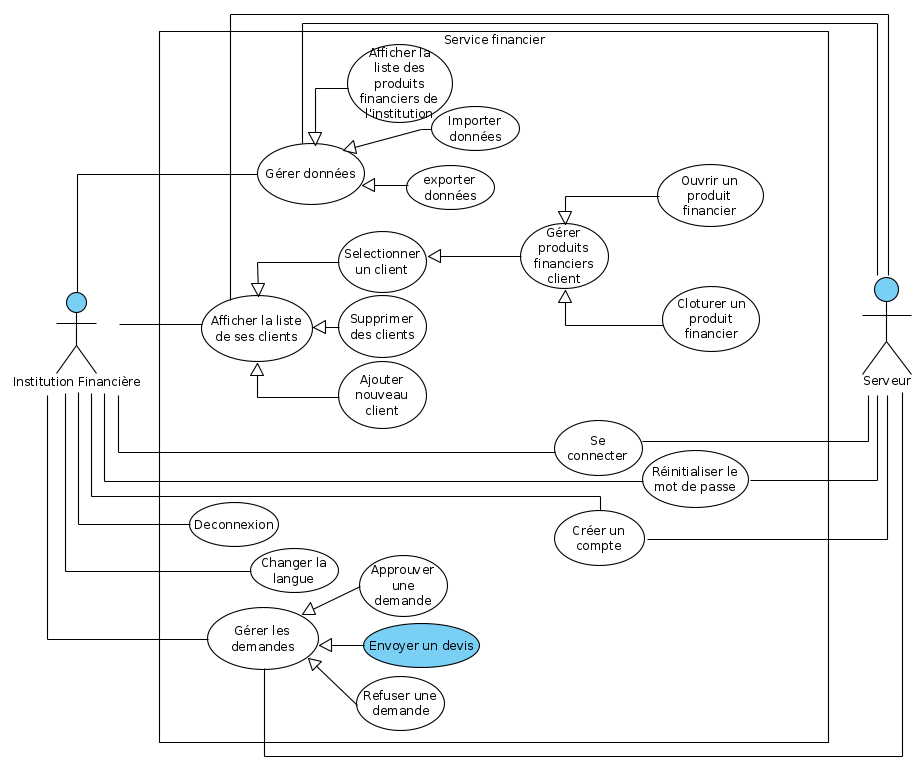
\includegraphics[scale=0.3]{img/UseCaseBanque.png}
        \caption{Use case de l'application banque pour l'extension assurance}
        \label{fig1}
        \end{figure}

    \paragraph{}Le use case de la partie banque n’ajoute que le cas “Envoyer un devis” qui est une spécification de gérer les demandes. Il sera néanmoins détaillé comme les autres à part.


\end{document}